\documentclass[a4paper,10pt]{article}

% Encoding and fonts
\usepackage[T1]{fontenc}
\usepackage[utf8]{inputenc}
\usepackage{newtxtext,newtxmath}

% Math / theorem support
\usepackage{amsmath}
\let\openbox\relax
\usepackage{amsthm}

% Graphics / TikZ / tkz packages
\usepackage{tikz}
\usetikzlibrary{arrows.meta, positioning, calc}
\usepackage{tkz-tab}
\usepackage{tkz-graph}

% Layout, code highlighting, misc
\usepackage[a4paper, margin=2cm]{geometry}
\usepackage{multicol}
\usepackage{graphicx}
\usepackage{xcolor}
\usepackage{caption}
\usepackage{minted}
\usepackage{booktabs}
\usepackage{multirow}
\usetikzlibrary{trees,positioning,arrows,shapes,automata}
% Theorem environments
\newtheorem{theorem}{Theorem}
\newtheorem{lemma}{Lemma}
\newtheorem{definition}{Definition}


\begin{document}

    \title{Lower Bounds on a Memory-Constrained Bidirectional Enumerator}
    \author{Ramillon Hugo, Michael Raskin}
    \date{}
    \maketitle

    \tableofcontents

\space

       \begin{abstract} 
            we study the relation between the time needed and the memory available for a specifically chosen sequence of operations, in this case the enumeration of n elements in a unidirectional enumerator. Our objective is twofold: first, to establish a general lower bound on the performance of any bidirectional enumerator operating within bounded memory; second, to construct explicit enumerators that closely approach these bounds after deamortization. We consider three distinct memory regimes—constant memory $\Theta(1)$, linear memory $\Theta(n)$, and logarithmic memory $\Theta(\log n)$—and show that in each case, the work per operation can match the theoretical lower bounds up to tight asymptotic factors.

            To unify these regimes, we introduce a novel relationship that governs the trade-off between memory usage and computational cost. We rigorously prove this relationship and use it to derive an optimality framework applicable to all three cases. Our approach includes a detailed analysis of the recursion underlying the enumeration process, focusing on its optimal segments. This analysis is supported by empirical data, validating the theoretical predictions and guiding the fine-tuning of the recursive structure.

            We implemented the resulting algorithms in Python, producing practical enumerators that come with provable guarantees on both average throughput and worst-case latency. Our work provides a comprehensive and practically viable framework for designing nearly optimal bidirectional enumerators under strict memory constraints.
        \end{abstract}

        \section{Introduction}

Efficient enumeration of data under memory constraints is a fundamental problem with significant implications in both theory and practice. We study the problem of enumerating a sequence in both forward and backward directions using sublinear memory, and we quantify the recomputation cost required to support backward traversal. This is especially relevant for unidirectional data structures such as hashchains, where backward traversal is not natively supported.

To illustrate this, consider a sequence of commits in a Git repository:
\[
\text{Commit A} \rightarrow \text{Commit B} \rightarrow \text{Commit C}
\]
Each commit includes the hash of its predecessor. In such structures, forward traversal is straightforward: from Commit~A one can derive Commit~B, and then Commit~C. However, given only Commit~C, reconstructing Commit~B is infeasible because cryptographic hash functions are one-way. Thus, backward traversal requires storing intermediate states, and a hashchain provides precisely the forward-only behavior that characterizes constrained enumeration models.

In constrained environments such as streaming or external memory models, one cannot store all intermediate states and must rely on sparse checkpointing to simulate backward movements. Our objective is to quantify the optimal tradeoff between memory usage and backward traversal cost, and to construct algorithms that achieve this optimal tradeoff.

This problem has been studied from various perspectives for a long time. Early results by Munro and Paterson~\cite{munro1980selection} and Beame~\cite{beame1991tradeoff} show that any sequential algorithm operating with sublinear memory must pay a superlinear computational cost. Vitter’s survey~\cite{vitter1999external} outlines the challenges of constrained I/O, which inspire the structural constraints considered in our model. Brodal and Fagerberg’s lower bounds for external memory dictionaries~\cite{brodal1999lower} motivate the search for fundamental limits under restricted memory. Sparse checkpointing, central to our approach, is discussed in their informal note~\cite{brodal1999kk} and finds a practical counterpart in Filliâtre’s backtracking iterators~\cite{filliatre2006backtracking}.

We formalize these principles through a recursive cost model that captures the tension between forward progress and backward traversal under memory constraints. From a complexity-theoretic perspective, our work relates to memory-limited sketching~\cite{alon1999frequency} and to automata-theoretic enumeration~\cite{moscowjournal2020linearorders}. The concept of bidirectional leveled enumerators~\cite{hal-03197935} further motivates our model.

\paragraph{Contributions.} In this paper:
\begin{enumerate}
    \item We define bidirectional enumeration with $k$ stored checkpoints and the associated recomputation cost $T(n,k)$.
    \item We show that $T(n,k)$ satisfies an optimal recurrence, and we derive a closed-form solution.
    \item We establish matching lower bounds, proving optimality.
    \item We establish new algorithms to have more or less the same complexity has our theoretical lower bounds
\end{enumerate}

\section{Searching for a Recurrence Matching the Lower Bound}

        \subsection{The recurrence and correspondence with our model}

            \subsubsection*{Establishing a First Recurrence}

                \paragraph{Writing the recurrence}

                We now formalize the problem. Let $T(n,k)$ denote the minimal cost required to enumerate a sequence of size $n$ in reverse order using at most $k$ memory cells, where $1 \le k \le n$. The goal is to compute the enumeration while minimizing the total amount of recomputation.

A memory cell stores an \emph{anchor}, i.e., a saved state of the unidirectional enumerator at a position $x \in \{1,\dots,n\}$. Placing an anchor at $x$ costs $x$ steps, since reaching $x$ requires forward traversal from the beginning of the sequence. Once placed, the anchor allows reverse enumeration to resume from $x$ without recomputing the prefix.

Placing an anchor at $x$ divides the enumeration into two subproblems. The left part, of length $x-1$, can still use all $k$ memory cells, whereas the right part, of length $n-x$, can only use the remaining $k-1$ cells. This yields the recurrence
\begin{equation}\label{eq:recurrence1}
    T(n,k) \;=\; \min_{1 \le x \le n} \bigl( x \;+\; T(x-1,k) \;+\; T(n-x,k-1) \bigr),
\end{equation}
where the term $x$ accounts for reaching the anchor, and the two recursive terms correspond to the left and right subproblems. This recurrence captures precisely the trade-off between memory usage and recomputation. Standard boundary conditions are
\[
T(0,k)=0,\qquad T(n,1)=\frac{n(n+1)}{2},\qquad T(n,n)=n.
\]

                    

            \subsubsection*{Verifying the Validity of the Recurrence}
To verify the correctness of the recurrence from the previous section, we analyze its behavior on small, tractable values of \(n\) and \(k\), which also serve as a basis for inductive proofs.

\paragraph*{Case 1: \(n = 1\), arbitrary \(k > 0\)}  
\[
T(1, k) = 1 + T(0, k) + T(0, k - 1) = 1
\]

\paragraph*{Case 2: \(k = 1\), arbitrary \(n\)}  
\[
T(n, 1) = n + T(n - 1, 1) = \sum_{i=1}^{n} i = \frac{n(n + 1)}{2},
\]
matching the expected cases cost under memory limitation.

\paragraph*{Inductive Proof of the Recurrence Validity}

Having verified the base cases, we now prove by induction that:

Assume that for all \(m < n\) and valid \(k\),
\[
T(m, k) = \min_{1 \le x \le m} \bigl( x + T(x-1, k) + T(m-x, k-1) \bigr)
\]
correctly gives the minimal enumeration cost.

\paragraph*{Induction Step}  
Consider a sequence of size \(n\) and an optimal first anchor \(1 \le x \le n\). By the hypothesis, \(T(x-1, k)\) and \(T(n-x, k-1)\) are minimal for the left and right subsequences. Therefore, the total cost is
\[
x + T(x-1, k) + T(n-x, k-1),
\]
and minimizing over all \(x\) gives
\[
T(n, k) = \min_{1 \le x \le n} \bigl( x + T(x-1, k) + T(n-x, k-1) \bigr).
\]

\paragraph*{Conclusion}  
By induction, the recurrence correctly models the minimal enumeration cost for all \(n \ge 1\) and valid \(k\), establishing the correctness of the model for further analysis.

\subsubsection*{Optimality of the Recurrence}

We prove that
\[
T(n,k)=\min_{1 \le x \le n} \bigl( x + T(x-1,k) + T(n-x,k-1) \bigr)
\]
indeed gives the minimal cost for bidirectional enumeration.

\begin{lemma}
For every $n \ge 1$ and $k \ge 1$, $T(n,k)$ equals the optimal cost of enumerating $[1,n]$ with~$k$ memory cells.
\end{lemma}

\begin{proof}
Let $S^*$ be an optimal strategy of cost $C^*$ for $(n,k)$. Since $k \ge 1$ and $n \ge 1$, $S^*$ must place an anchor at some $x \in \{1,\dots,n\}$, at cost $x$. Removing this anchor yields two subproblems of sizes $x-1$ and $n-x$, which use $k$ and $k-1$ memory cells respectively. Thus
\[
C^* = x + C^*_{\mathrm{L}} + C^*_{\mathrm{R}}.
\]

By Bellman’s optimality principle~\cite{bellman1957dynamic, bertsekas1995dynamic}, the restrictions of $S^*$ to the two subproblems are themselves optimal; otherwise they could be replaced by cheaper solutions, contradicting the optimality of $S^*$. Hence
\[
C^*_{\mathrm{L}} = T(x-1,k),\qquad C^*_{\mathrm{R}} = T(n-x,k-1),
\]
so
\[
C^* = x + T(x-1,k) + T(n-x,k-1).
\]

Since the right-hand side is one of the candidates in the minimization defining $T(n,k)$, we obtain $C^* \ge T(n,k)$. The reverse inequality follows from constructing a strategy that attains the minimum, so $C^*=T(n,k)$.
\end{proof}
These values illustrate how additional memory cells reduce recomputation cost: while $T(n,1)=\Theta(n^2)$, even a small number of memory cells (e.g., $k=2$ or $k=3$) yields a substantial improvement.
\begin{table}[H]
\centering
\caption{Example values of $T(n,k)$ for small $n$ and $k$.}
\label{tab:small-values}
\medskip
\begin{tabular}{c|ccccc}
\toprule
$n \backslash k$ & $1$ & $2$ & $3$ & $4$ & $5$ \\
\midrule
$1$ & $1$ & $1$ & $1$ & $1$ & $1$ \\
$2$ & $3$ & $2$ & $2$ & $2$ & $2$ \\
$3$ & $6$ & $4$ & $3$ & $3$ & $3$ \\
$4$ & $10$ & $6$ & $5$ & $4$ & $4$ \\
$5$ & $15$ & $8$ & $7$ & $6$ & $5$ \\
$6$ & $21$ & $11$ & $9$ & $8$ & $7$ \\
\bottomrule
\end{tabular}
\end{table}

\subsection{Equivalence of the other methods with our model}
Let us assume that there exists a better method, characterized by a more efficient recurrence.  
In this new model, computing a backward enumeration requires obtaining the value at position $n$, then at $n-1$, and so on.  
However, according to the definition of a hash chain, computing the value at position $n$ requires knowing the value at position $n-1$.  
In a memory-limited environment, it is impossible to start from the beginning, compute all intermediate values, and then simply return the reversed sequence.  
Therefore, any algorithm must store intermediate values. With $k$ available memory cells, at most $k$ such values can be stored.  

The central question is: which $k$ positions should be stored to minimize recomputation?  
To achieve optimal performance, one must strategically select certain values of the hash chain as checkpoints.  
Any choice of $k$ checkpoint positions induces a decomposition of the sequence.  
To evaluate the computational cost, note that reaching each checkpoint requires forward traversal from the start (or from a previous checkpoint).  
This recursive structure is precisely captured by our recurrence $T(n, k)$, which determines the optimal placement of checkpoints.  

Consequently, any algorithm for backward enumeration effectively reduces to choosing these $k$ positions optimally—a problem our model solves.  
Therefore, no alternative method can outperform the bound defined by $T(n, k)$.



\section{Study of the recursion}

When \(n\) increases, we observe that \(T(n,k)\) grows faster and faster.  
Let us call \(i\) the marginal cost between \(T(n,k)\) and \(T(n+1,k)\).  
Since we believe this marginal cost changes throughout the recursion, we define a sequence \(n_k(i)\), which marks the values of \(n\) where the marginal cost increases.

We now introduce a property \(P(n)\): there exists a value \(i\) such that the marginal cost between \(T(n,k)\) and \(T(n+1,k)\) is \(i\), and this value was determined at step \(n_k(i)\).

\paragraph*{Initialization for \(n < k\).}
When \(n < k\), we have enough anchors to enumerate all solutions, hence
\[
T(n,k) = n .
\]
For \(n+1 \le k\), the same holds:
\[
T(n+1,k) = n+1,
\]
so the marginal cost is \(i = 1\).

However, when \(n = k\),
\[
T(k,k) = k,
\]
but
\[
T(k+1,k) \neq k+1
\]
because memory is no longer sufficient.  
Thus, the first increase point is
\[
n_k(i) = k+1.
\]

\paragraph*{Inductive step.}
Assume \(P(n)\) holds: there exists a marginal cost \(i\) between \(T(n,k)\) and \(T(n+1,k)\), and that cost was fixed at \(n_k(i)\).

To prove \(P(n+1)\), observe that either:

1. The marginal cost remains the same:
   \[
   T(n+2,k) = T(n+1,k) + i,
   \]
   or

2. The marginal cost increases.  
   In this case we denote the new cost by \(i'\), and \(n+2\) becomes a member of the sequence \(n_k(i')\).

For \(n \in [n_k(i),\, n_k(i')]\), the recursion behaves linearly:
\[
T(n,k) = T(n_k(i),k) + i \times (n - n_k(i)).
\]

Let \(l = i' - i\) be the increment between two successive marginal prices.  
We claim that **always \(l = 1\)**.  
This can be proven by induction on \(k\), based on the structure of the recursion.

Proving \(l = 1\)

\paragraph*{Base case \(k = 1\).}
With no anchors, every new value of \(n\) requires recomputing the entire problem.  
Thus the marginal cost always increases by exactly one:
\[
n_1(i') - n_1(i) = 1.
\]

\paragraph*{Inductive step.}
Assume the statement holds for some \(k\).  
We prove it for \(k+1\).

From the definition of the recursion,
\[
T\bigl(n_{k+1}(i),\, k+1\bigr)
  = x^* + T(x^*-1,k+1) + T\bigl(n_{k+1}(i)-x^*,k\bigr),
\]
meaning that a \((k+1)\)-anchor problem eventually reduces to a \(k\)-anchor problem whose marginal cost increases by exactly 1.

If \(l \ne 1\), then the subproblems with \(k\) anchors would exhibit a marginal increase different from 1, contradicting the induction hypothesis.  
Therefore \(l = 1\) for all \(k\).

---

 Graphical interpretation

When representing the recursion as a graph (for example \(T(6,2)\)), the last three vertices after the anchor form a subproblem of size \(T(3,1)\):
\begin{center}
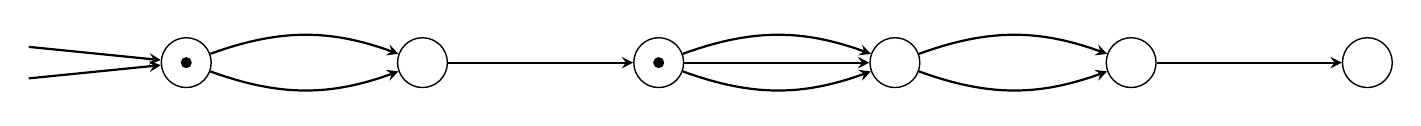
\begin{tikzpicture}
  \GraphInit[vstyle=Normal]
  \SetGraphUnit{3}
  \SetVertexNoLabel

  \Vertex{V1}
  \fill (V1) circle (2pt);
  \EA(V1){V2}
  \EA(V2){V3}
  \fill (V3) circle (2pt);
  \EA(V3){V4}
  \EA(V4){V5}
  \EA(V5){V6}

  \draw[->,>=stealth,thick] (-2,0.2) -- (V1);
  \draw[->,>=stealth,thick] (-2,-0.2) -- (V1);

  \tikzset{EdgeStyle/.style={->,>=stealth,bend left=20}}
  \Edge(V1)(V2)
  \tikzset{EdgeStyle/.style={->,>=stealth,bend right=20}}
  \Edge(V1)(V2)

  \tikzset{EdgeStyle/.style={->,>=stealth}}
  \Edge(V2)(V3)

  \tikzset{EdgeStyle/.style={->,>=stealth,bend left=20}}
  \Edge(V3)(V4)
  \tikzset{EdgeStyle/.style={->,>=stealth,bend right=0}}
  \Edge(V3)(V4)
  \tikzset{EdgeStyle/.style={->,>=stealth,bend right=20}}
  \Edge(V3)(V4)

  \tikzset{EdgeStyle/.style={->,>=stealth,bend left=20}}
  \Edge(V4)(V5)
  \tikzset{EdgeStyle/.style={->,>=stealth,bend right=20}}
  \Edge(V4)(V5)

  \tikzset{EdgeStyle/.style={->,>=stealth}}
  \Edge(V5)(V6)
\end{tikzpicture}
\end{center}
Representation of \(T(3,1)\):

\begin{center}
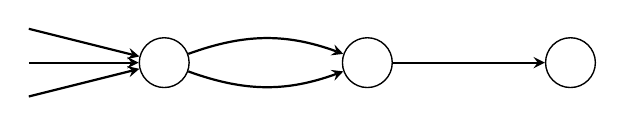
\begin{tikzpicture}[scale=0.86]
  \GraphInit[vstyle=Normal]
  \SetGraphUnit{3}
  \SetVertexNoLabel

  \Vertex{V1}
  \EA(V1){V2}
  \EA(V2){V3}

  \draw[->,>=stealth,thick] (-2,0.5) -- (V1);
  \draw[->,>=stealth,thick] (-2,0) -- (V1);
  \draw[->,>=stealth,thick] (-2,-0.5) -- (V1);

  \tikzset{EdgeStyle/.style={->,>=stealth,bend left=20}}
  \Edge(V1)(V2)
  \tikzset{EdgeStyle/.style={->,>=stealth,bend right=20}}
  \Edge(V1)(V2)

  \tikzset{EdgeStyle/.style={->,>=stealth}}
  \Edge(V2)(V3)
\end{tikzpicture}
\end{center}
Recalling the recurrence
\[
T(n,k) = \min_{1 \le x \le n} \left( x + T(x-1, k) + T(n-x, k-1) \right),
\]
we can intuitively expect that a minimizer \(x^*\) of \(T(n_k(i),k)\) is
\[
x_k(i) = n_k(i-1),
\]
because we first visit the most expensive prefix of size \(n_k(i-1)\), place an anchor, and then enumerate the remaining part.

We now prove the property
\[
P(i): x_k(i) = n_k(i-1)
\]
by induction on \(i\).

\paragraph*{Initialization: \(i=1\).}
The minimizer of \(T(n_k(1),k)\) is \(n_k(0)=1\), since the first element that leaves marginal cost \(0\) is exactly the first element we wish to enumerate. Hence the base case holds.

\paragraph*{Induction step.}
Assume \(P(i)\) holds, i.e., \(x_k(i)=n_k(i-1)\). We prove that it remains true for \(i+1\).

To compute \(T(n_k(i+1), k)\), we first compute \(T(n_k(i), k)\), then the remaining portion
\[
T(n_k(i+1)-n_k(i), k-1).
\]
A first attempt would be
\[
T(n_k(i+1), k) = T(n_k(i), k) + T(n_k(i+1)-n_k(i), k-1).
\]
However, after using all our anchors, we cannot compute the second term without redoing the entire walk. Therefore, a correction term \(n_k(i)\) must be added:
\[
\begin{aligned}
T(n_k(i+1), k) = T(n_k(i), k) + T(n_k(i+1)-n_k(i), k-1)&  // + n_k(i).
\end{aligned}
\]
Since we already have an anchor at position \(n_k(i)\), we can optimize the first term:
\[
T(n_k(i+1), k)
  = T(n_k(i)-1, k) + T(n_k(i+1)-n_k(i), k-1) + n_k(i).
\]
This shows that the same minimizer structure continues to hold, so
\[
x_k(i+1) = n_k(i).
\]
Thus, by induction, \(x_k(i) = n_k(i-1)\) for every \(i\).

\bigskip

We now prove that
\[
n_k(i) = n_k(i-1) + n_{k-1}(i).
\]
Using the recurrence and the established minimizer, we have
\[
T(n_k(i), k)
  = n_k(i-1) + T(n_k(i)-1, k) + T(n_k(i)-n_k(i-1), k-1).
\]
Suppose, for contradiction, that
\[
n_k(i) \neq n_k(i-1) + n_{k-1}(i).
\]
The expression above is optimal, and in particular the term
\[
T(n_k(i)-n_k(i-1), k-1)
\]
must not contain an element of marginal cost strictly greater than \(i\). Otherwise, \(T(n_k(i), k)\) would itself contain a marginal cost larger than \(i\), contradicting the definition of \(n_k(i)\). Hence
\[
n_{k-1}(i) = n_k(i) - n_k(i-1),
\]
and therefore
\[
n_k(i) = n_k(i-1) + n_{k-1}(i).
\]
This completes the proof.

Since this recurrence is identical to Pascal's identity \cite{graham1994concrete}
\[
\binom{a}{b} = \binom{a-1}{b} + \binom{a-1}{b-1},
\]
and since the initial conditions match, we obtain
\[
n_k(i) = \binom{i + k - 1}{k}.
\]

From this we derive the closed form of \(T(n_k(i),k)\):
\[
T(n_k(i), k) = k \times \binom{i + k - 1}{k+1} + i.
\]

\paragraph*{Proof by induction.}

\paragraph*{Double initialization: \(i=1\), and \(k=1\) / \(k=2\).}
We need two initializations on \(k\) because the summation used above holds only for \(k \ge 2\).

\medskip
\noindent\textbf{Initialization on \(i=1\).}
\[
T(n_k(1), k)
  = k \times \binom{1 + k - 1}{k+1} + 1
  = k \times \binom{k}{k+1} + 1
  = 0 + 1
  = 1.
\]

\medskip
\noindent\textbf{Initialization on \(k=1\).}
Since \(n_1(i) = i\), we have
\[
T(n_1(i), 1) = 1 \times \binom{i}{2} + i.
\]
But
\[
T(i,1) = \frac{i(i+1)}{2}, \quad \text{and} \quad \binom{i}{2} = \frac{i(i-1)}{2}.
\]
Hence
\[
\frac{i(i+1)}{2} = \frac{i(i-1)}{2} + i,
\]
so the formula holds.

\paragraph*{Induction step.}

Assume for fixed \(i\ge 1\) and \(k\ge 1\) that
\[
T(n_k(i), k) = k\times \binom{i + k - 1}{k+1} + i.
\]
We prove it holds for \(i+1\):
\[
\small
\begin{aligned}
T(n_k(i+1),k)
  &= n_k(i) + T(n_k(i)-1,k) + T(n_{k-1}(i+1),k-1) \\
  &= \binom{i+k-1}{k} + k \times \binom{i+k-1}{k+1} \\
  &+ i - i + (k-1)\times \binom{i + k - 1}{k} + i + 1 \\
  &= k \times \bigl( \binom{i + k - 1}{k} + \binom{i + k - 1}{k+1} \bigr) + i + 1 \\
  &= k \times \binom{i + k}{k+1} + i + 1.
\end{aligned}
\]

Now for \(k \to k+1\), we have
\[
\small
\begin{aligned}
T(n_{k+1}(i),k+1)
  &= n_{k+1}(i-1) + T(n_{k+1}(i-1)-1,k+1) + &\\ T(n_k(i),k) \\
  &= \binom{i+k-1}{k+1} + (k+1)\times \binom{i+k-1}{k+2} \\
  &+ i - i+ k\times \binom{i + k - 1}{k + 1} + i \\
  &= (k+1)\times\bigl( \binom{i+k-1}{k+1} + \binom{i+k-1}{k+2} \bigr) + i \\
  &= (k+1) \times \binom{i + k}{k + 2} + i.
\end{aligned}
\]
Thus the statement is proven by induction.

\section{Asymptotic bounds under memory constraint}

We write
\[
f(n) \sim g(n)
\]
to denote that \( f(n) \) is asymptotically equivalent to \( g(n) \), that is,
\[
\lim_{n \to \infty} \frac{f(n)}{g(n)} = 1.
\]
This means that \( f(n) \) and \( g(n) \) grow at the same rate as \( n \to \infty \).


\subsection{Lower Bound for \( \theta(1) \) Memory}

We seek to establish a lower bound on the cost function \( T(n, k) \), which represents the number of forward steps performed by a bidirectional enumerator operating with \( k \) memory cells. Our approach is to analyze a structured recursive strategy that models the behavior of such an enumerator under memory constraints. This structured strategy, while idealized, provides a tractable framework from which we can derive a lower bounds.

Simultaneously, we introduce the function \( i_k(n) \), which denotes the cost increment at position \( n \). Previously, we showed that the value \( i \) corresponds to the marginal cost at specific positions \( n_k(i) \), and that these \( n_k(i) \) serve as the change points for \( i_k(n) \). In what follows, we aim to demonstrate that \( n_k(i) \sim i^k \), and consequently, \( i_k(n) \sim n^{1/k} \).

For fixed \(k \ge 1\), the sequence
\[
n_k(i) = \binom{k+i-1}{k}
\]
satisfies
\[
n_k(i) \sim \frac{i^k}{k!} \qquad \text{as } i \to \infty.
\]
In particular, for \(n = n_k(i)\), we have \(i \sim n^{1/k}\).

We expand the binomial coefficient as a polynomial in \(i\):
\[
\binom{k+i-1}{k}
= \frac{i(i+1)\cdots(i+k-1)}{k!}
= \frac{1}{k!}\bigl(i^k + \beta_{k-1} i^{k-1} + \cdots + \beta_0\bigr),
\]
where the constants \(\beta_j\) depend only on \(k\). Therefore,
\[
\binom{k+i-1}{k}
= \frac{i^k}{k!}\left(1 + \frac{\beta_{k-1}}{i} + \cdots + \frac{\beta_0}{i^k}\right).
\]
As \(i \to \infty\), all negative powers of \(i\) vanish, which gives
\[
\binom{k+i-1}{k} = \frac{i^k}{k!}\,(1 + o(1)).
\]
Hence,
\[
n_k(i) = \binom{k+i-1}{k} \sim \frac{i^k}{k!} \cite{flajolet2009analytic}.
\]

Now as long as $n$ is always between two $n_k(i)$ and $n_k(i)+1$ we can say that \(n \sim n_k(i)\). Since \(i \mapsto \binom{k+i-1}{k}\) is strictly increasing for \(i \ge 1\), we may invert asymptotically:
\[
n = \frac{i^k}{k!}(1+o(1))
\quad\Longrightarrow\quad
i^k \sim k! \, n.
\]
Taking \(k\)-th roots yields
\[
i \sim (k!)^{1/k}\,n^{1/k} \sim n^{1/k}.
\]
Thus \(i\) grows like \(n^{1/k}\), completing the proof.

Substituting into the expression for \( T(n_k(i), k) \), we get:
\begin{align*}
T(n_k(i), k) 
&= k \times \frac{(i-1)i(i+1)\cdots(i+k-1)}{(k+1)!} + i \\[2mm]
&= n_k(i) \cdot \frac{k(i-1)}{k-1} + i \\[1mm]
&\sim \frac{i^{k+1}}{(k+1)!} \\[1mm]
&\sim \frac{(k!)^{1+1/k}}{(k+1)!}\, n^{1+1/k} \\[1mm]
&= C\, n^{1+1/k}, \quad C = \frac{(k!)^{1/k}}{k+1}.
\end{align*}

Therefore, we conclude:
\[
T(n_k(i), k) \in \theta\left(n^{1 + \frac{1}{k}}\right).
\]

\subsection{Lower bound for \( \theta(n) \)}
This one is obvious
\ref{eq:recurrence1}
\[
T(n, n) = 1 + T(0,n) + T(n-1,n-1) = \sum_{k=1}^{n} 1 = n,
\]
we have \( \theta(n) \) time complexity.

\subsection{Lower Bound for \( \theta(\log n) \) Memory}

Based on the recursive definition of \( T(n,k) \), we consider the case \( k = \log n \). 
For some integer \( i \), we have
\[
T\big(n_{\log n}(i), \log n\big) \leq T(n, \log n) \leq T\big(n_{\log n}(i+1), \log n\big).
\]

For
\[
n_{\log n}(i) = \binom{\log n + i - 1}{\log n},
\]
solving asymptotically for \( i \) in terms of \( n \) gives
\[
n_{log n}(i) \sim \frac{ i^{\log n}}{(\log n)!}
\quad \Longrightarrow \quad
i^{log n} \sim log(n)! n
\]

Using Stirling’s approximation,
\[
(\log n)! = \Theta\big( (\log n)^{\log n} \big),
\]
we get
\[
i \sim \Theta((log n)^{\frac{log n}{log n}} \times n^{\frac{1}{log n}})
  = \Theta\!\left( n^{\frac{1}{\log n}} \cdot \log n \right).
\]

Since
\[
n^{\frac{1}{\log n}} = e^{\frac{\ln n}{\log n}} \to \text{constant as } n \to \infty,
\]
we conclude
\[
i = \Theta(\log n).
\]

Then \(n_{\log n}(i) = \Theta(n)\).

\paragraph{Asymptotic evaluation of \(T(n_{\log n}(i), \log n)\).} Using the recurrence,
\[
T(n_{\log n}(i),\log n) = n_{\log n}(i) \cdot \frac{\log n + i - 1}{\log n - 1} + i
= \Theta(n_{\log n}(i) \cdot i + i)
= \Theta(n \log n + \log n)
= \Theta(n \log n).
\]

Hence, using \(\Theta(\log n)\) memory, the cost satisfies
\[
T(n, \Theta(\log n)) = \Theta(n \log n),
\]

We now have a lower bound for $\Theta(log(n))$
\section{Algorithms Which Approach Our Theoretical Bounds}

\subsection{Algorithm for $\Theta(n)$~\cite{filliatre2006backtracking}}

This algorithm stores every position during the forward traversal, allowing
exact backward steps in constant time per operation.

\paragraph{Data Structures.} The algorithm maintains:
\begin{itemize}
    \item \texttt{current}: the current enumerator state;
    \item \texttt{distance}: the distance from the start;
    \item \texttt{saved\_positions}: a stack of previously visited positions.
\end{itemize}

The algorithm is straightforward. During the forward traversal, each visited
state is pushed onto the stack. During the backward traversal, states are
popped from the stack to restore the previous position.


\textbf{Time Complexity:} $\mathcal{O}(n)$ total, $\mathcal{O}(1)$ per operation, using $\mathcal{O}(n)$ space.

\begin{table}[H]
\centering
\caption{Measured cost for increasing distances $n$ (expected $O(n)$).}
\label{tab:linear-scaling}
\medskip
\begin{tabular}{c|c|c|c}
\toprule
Distance $n$ & Operations& Theoretical & Ratio \\
\midrule
$100$  & $100$  & $100$  & $1.000$ \\
$400$  & $400$  & $400$  & $1.000$ \\
$900$  & $900$  & $900$  & $1.000$ \\
$1600$ & $1600$ & $1600$ & $1.000$ \\
\bottomrule
\end{tabular}
\end{table}



\subsection{Algorithm for $\Theta(\log n)$ Memory}

We now describe a bidirectional enumeration algorithm that operates with
$\Theta(\log n)$ memory and achieves a total cost of $\Theta(n \log n)$,
matching the lower bound established in Section~4.3 up to constant factors.

\paragraph{High-level intuition.}
Since the target time complexity is $\Theta(n \log n)$, it is natural to organize
the enumeration around a hierarchical structure reminiscent of a binary tree.
Conceptually, we consider an implicit tree whose root corresponds to position~$0$.
For each node at position $x$, the left child corresponds to the next power of two
greater than $x$, while the right child corresponds to $x$ plus the smallest
unused power of two. Iterating this construction yields a tree that spans all even
positions and reflects the exponential spacing inherent to powers of two.

However, maintaining checkpoints only at positions $1,2,4,8,\ldots$ is insufficient
in practice. Indeed, the gap between two consecutive powers of two may be large
(e.g., between $256$ and $512$), leading to excessive recomputation during backward
steps.

\paragraph{Checkpoint spacing strategy.}
To address this issue, the algorithm dynamically maintains a set of
well-spaced checkpoints during the forward traversal.
First, an anchor is added systematically at every position that is a power of two;
this operation takes $\Theta(1)$ time and guarantees a logarithmic upper bound on
the number of anchors.

In addition, the algorithm maintains two auxiliary quantities:
\begin{itemize}
  \item the \emph{marginal distance}, defined as the distance between the current
  position and the most recently placed checkpoint;
  \item the \emph{minimum inter-checkpoint distance}, i.e., the smallest distance
  between any two consecutive checkpoints currently stored.
\end{itemize}
Both quantities can be updated in $\Theta(1)$ time, since checkpoints are introduced
at powers of two and only local adjustments are required.

Whenever the marginal distance exceeds the minimum inter-checkpoint distance,
the algorithm removes the checkpoint corresponding to the largest index realizing
this minimum distance and replaces it with a new checkpoint at the current position.
This replacement rule guarantees that checkpoints remain evenly distributed along
the traversal, preventing the formation of large gaps.

\paragraph{Backward traversal.}
During backward enumeration, two cases arise.
If the current position is not a checkpoint, the algorithm recomputes the previous
state starting from the most recent checkpoint.
If the current position coincides with a checkpoint, the algorithm recomputes an
optimal set of checkpoints by inserting new ones at midpoints between the current
position and earlier checkpoints along the path. Conceptually, the current checkpoint
is removed, and the algorithm attempts to reinsert checkpoints so as to preserve the
spacing invariant.

If no position is available between two consecutive checkpoints, the algorithm
recursively searches earlier intervals. When no further insertion is possible,
the anchor corresponding to the root is discarded. At this stage, the number of
remaining elements is bounded by $O(\log n)$, and the remaining backward traversal
can be completed with negligible additional cost.

\paragraph{Complexity analysis.}
At all times, the algorithm stores at most $\Theta(\log n)$ checkpoints.
Each forward step performs only constant-time maintenance operations, while each
backward step triggers at most $\Theta(\log n)$ recomputation in the worst case.
Summed over the entire execution, this yields a total cost of $\Theta(n \log n)$,
in accordance with the theoretical lower bound for $\Theta(\log n)$ memory.

\begin{center}
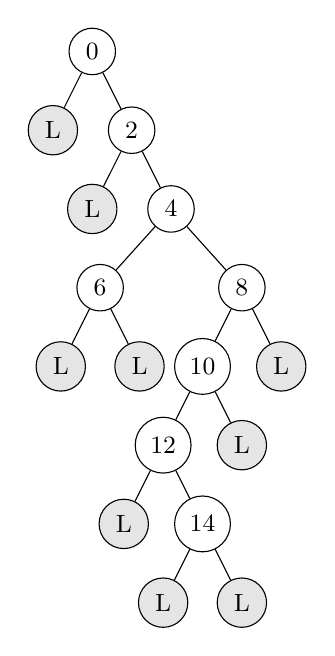
\begin{tikzpicture}[
  level 1/.style={sibling distance=10mm},
  level 2/.style={sibling distance=10mm},
  level 3/.style={sibling distance=18mm},
  level 4/.style={sibling distance=10mm},
  level distance=1cm,
  sibling distance=1cm,
  every node/.style={circle, draw, minimum size=0.2cm, font=\small},
  leaf/.style={fill=gray!20}
]

\node {0}
  child{
      node[leaf]{L}
    }
  child {
    node {2}
    child{
      node[leaf]{L}
    }
    child {
      node {4}
      child {  node{6} 
        child{node[leaf]{L}}
        child{node[leaf]{L}}
      }
      child {
        node {8}
        child {
          node {10}
          child {
            node{12}
            child{
              node[leaf]{L}
            }
            child { node {14}
                child{node[leaf]{L}}
                child{node[leaf]{L}}
            }
          }
          child{
              node[leaf]{L}
            }
        }
        child{
              node[leaf]{L}
            }
      }
    }
  };

\end{tikzpicture}
\end{center}


\begin{table}[H]
\centering
\caption{Experimental values of the cost for several $n$.}
\label{tab:experimental-values}
\medskip
\begin{tabular}{c c c c c}
\toprule
$n$ & $\log_2(n)$ & Operations & Theoretical bound & Ratio \\
\midrule
$128$  & $7$  & $223$  & $896$   & $0.249$ \\
$256$  & $8$  & $601$  & $2048$  & $0.293$ \\
$1024$ & $10$ & $2658$ & $10240$ & $0.260$ \\
$2048$ & $11$ & $6678$ & $22528$ & $0.296$ \\
\bottomrule
\end{tabular}
\end{table}



\subsection{Algorithm for $\Theta(1)$}

In this section, we briefly recall the idea behind the $\Theta(1)$-space bidirectional enumeration algorithm.  
\medskip

On the other hand, the bidirectional algorithm with $\Theta(n)$ memory remains very simple and follows a recursive strategy.

We rely on the classical combinatorial relation
\[
  n_k(i) = \binom{k + i - 1}{k},
\]
which tells us where the $k$ anchors should be placed.  
For each anchor, we store:
\begin{itemize}
    \item its current position in the enumeration, and
    \item the last index of this anchor that has already been placed.
\end{itemize}
With this information, performing a \texttt{next} operation is straightforward, as we can jump to the closest relevant anchor.

\medskip

Moreover, we maintain a small auxiliary table containing the \emph{next} $k$ anchors, so that we do not need to recompute combinatorial values at every step.  
If the current distance exceeds the limit given by the last stored anchor plus one element of this table, we shift all anchors forward: we move the last anchor, update its index, and compute the new value of the next anchor.

In the reverse direction (\texttt{previous} operation), we proceed symmetrically.  
Whenever an anchor becomes obsolete because it is too far ahead in the enumeration, we decrement its index and update its stored value accordingly.

\begin{table}[H]
\centering
\caption{Measured cost for several memory sizes $k$, compared to the theoretical bound $n^{1+1/k}$.}
\label{tab:k10-50-100}
\medskip
\begin{tabular}{c|c|c|c|c}
\toprule
$k$ & $n$ & Operations (ops) & $n^{1+1/k}$ & Ratio \\
\midrule
\multirow{4}{*}{$10$}
 & $32$   & $59$   & $45$   & $1.304$ \\
 & $512$  & $1765$  & $955$  & $1.847$ \\
 & $2048$  & $8006$  & $4390$  & $1.824$ \\
 & $4096$ & $17831$ & $9410$ & $1.895$ \\
\midrule
\multirow{4}{*}{$50$}
 & $32$   & $32$   & $34$   & $0.933$ \\
 & $512$  & $1007$  & $580$  & $1.736$ \\
 & $2048$  & $5344$  & $2385$  & $2.240$ \\
 & $4096$ & $11817$ & $4837$ & $2.2443$ \\
\midrule
\multirow{4}{*}{$100$}
 & $128$   & $32$   & $33$   & $0.966$ \\
 & $512$  & $1002$  & $545$  & $1.839$ \\
 & $2048$  & $4017$  & $2210$  & $1.817$ \\
 & $4096$ & $8111$ & $4451$ & $1.822$ \\
\bottomrule
\end{tabular}
\end{table}


\section*{Conclusion}
We have successfully achieved all of our initial objectives. We derived, analyzed, and rigorously proved a recursive formulation to model and minimize the cost of memory-constrained bidirectional enumeration:
\[
T(n, k) = \min_{1 \le x \le n} \left( x + T(x - 1, k) + T(n - x, k - 1) \right).
\]
This recurrence, $T(n, k)$, revealed a rich internal structure. By focusing on instances where the minimizing split point is unique, we uncovered several structural relationships—some of which were formally demonstrated and discussed throughout this article. These relationships provide significant insight into the behavior and progression of the recursion:
\begin{align*}
T(n_k(i), k) = k\times \binom{i + k - 1}{k+1} + i.
\end{align*}

Furthermore, these relationships allowed us to establish lower bounds on the cost function under three different memory regimes: $\Theta(1)$, $\Theta(n)$, and $\Theta(\log n)$. We proved that the corresponding time complexities are respectively
\[
\Theta\left(n^{1 + \frac{1}{k}}\right), \quad \Theta(n), \quad \text{and} \quad \Theta(n \log n).
\]

Finally, we proposed algorithms that approach these bounds, suggesting that our lower bounds are tight—or nearly tight—in practice.

\paragraph{Availability}
The code is available at:
https://github.com/hramillon/Lower-Bounds-on-a-Memory-Constrained-Backward-Bidirectional-Enumerator

\bibliographystyle{abbrv}
\bibliography{biblio}

\end{document}